\documentclass[handout]{beamer}
\usepackage[utf8]{inputenc}
\usepackage[T1]{fontenc}
\usepackage[french]{babel}
\usepackage{color}
\usepackage{fancyhdr}
\usepackage{lmodern}
\usepackage{makeidx}
\usepackage{graphicx}
\usepackage{amsmath}
\usepackage{amssymb}
\usepackage{mathrsfs}
\usepackage[bottom]{footmisc}
\usepackage{float}
\usepackage{listings}
\usepackage{textcomp}
\usepackage{verbatim}
\usepackage{ulem}
\usepackage{xcolor}

\lstset{language=Python,commentstyle=\color{gray},
	keywordstyle=\color{red},
	stringstyle=\color{blue},morekeywords={plt,np},
	breaklines=true,literate={é}{{\'e}}1}

\usetheme{ki}
\usefonttheme{serif}

\title{Formation \LaTeX}
\author{KI '022}
\institute{\color{white}Ecole des Ponts Paristech}
\date{\today}

\begin{document}

	\begin{frame}
		\titlepage
	\end{frame}

	\begin{frame}
		\frametitle{Sommaire}
		\setcounter{tocdepth}{1}
		\tableofcontents
	\end{frame}
\section{Introduction}

\begin{frame}{Qu'est ce que \LaTeX \ ?}
	\hspace*{-1cm}
	\begin{tabular}{c c c}
		 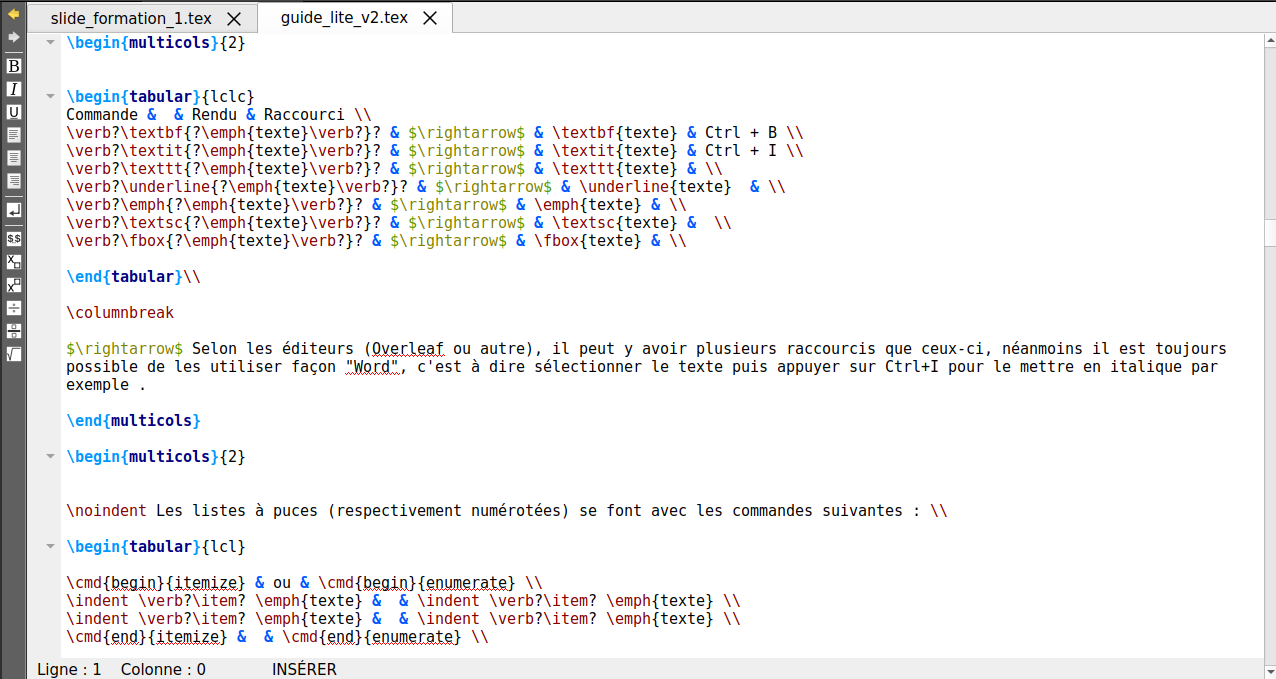
\includegraphics[scale=0.13]{ressources/latex_raw.png} & & 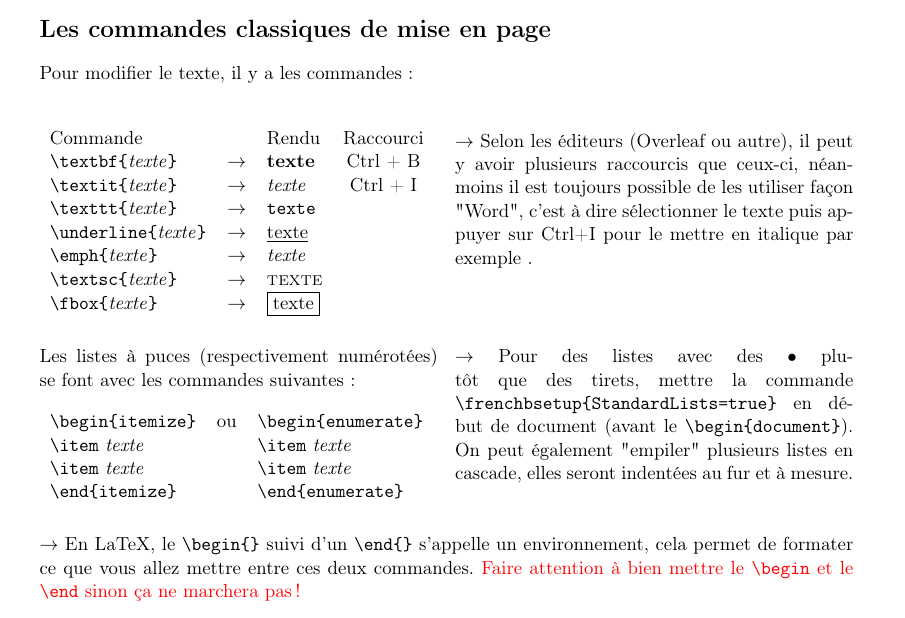
\includegraphics[scale=0.15]{ressources/latex_output.png}\\
		  Fichier.tex & $\longrightarrow$ &  Fichier PDF
	\end{tabular}
\end{frame}

\begin{frame}{Overleaf}
	\centering \url{https://fr.overleaf.com/}
	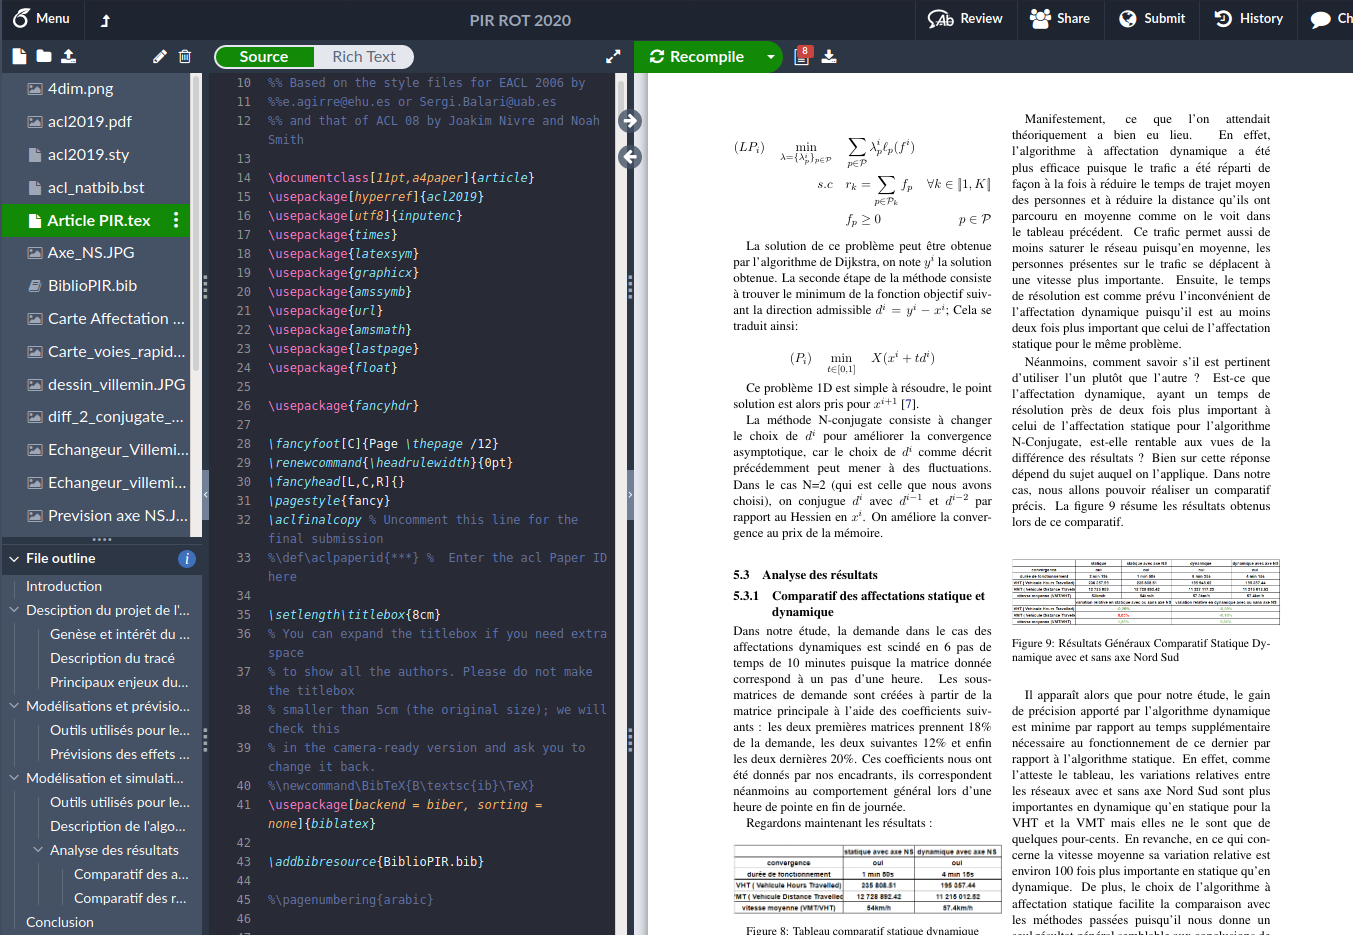
\includegraphics[scale=0.18]{ressources/overleaf.png}
\end{frame}
\section{Créer un premier document \LaTeX}
\begin{frame}{La base de tout document}
	\vspace*{-0.3cm}
	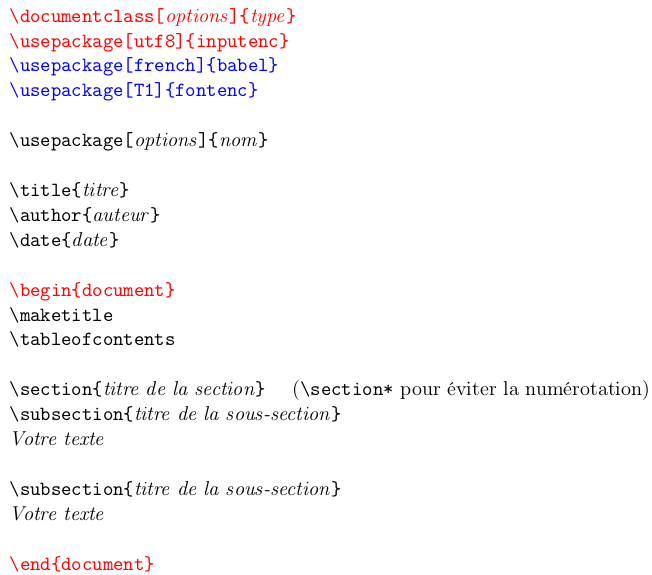
\includegraphics[scale=0.35]{ressources/basedoc}	
\end{frame}

\begin{frame}[fragile]{La commande}
En \LaTeX, tout passe par la commande, la forme générale étant:\\
\texttt{\textbackslash nom\_commande[\textit{option 1 = , option 2 =}]\{...\}}\\[0.5cm]

Par exemple avant tout document il faut mettre une ligne du type:\\
\texttt{\textbackslash documentclass[11pt,a4paper]\{article\}}\\[0.5cm]

Et la plupart du temps il y aura aussi:
\texttt{\textbackslash usepackage[option]\{nom\_du\_package\}}
\end{frame}

\begin{frame}{Structurer son document}
\begin{itemize}
	\item Faire apparaître le titre : \texttt{\textbackslash maketitle}
	\item Structure interne : \texttt{\textbackslash section\{\}}, \texttt{\textbackslash subsection\{\}}, ...
	\item Sans numérotation : \texttt{\textbackslash section*\{\}}
	
\end{itemize}
\vfill
$\longrightarrow$ Tout ça entre le \texttt{\textbackslash begin\{document\}} et le \texttt{\textbackslash end\{document\}} !!!
\end{frame}

\begin{frame}
	\hspace*{-0.5cm}
	\vspace*{-0.5cm}
	\begin{columns}
		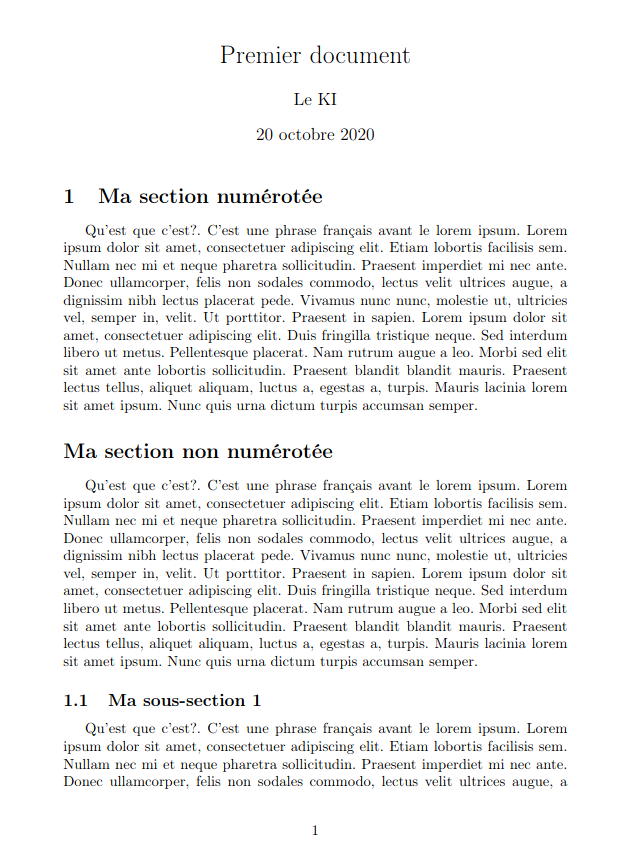
\includegraphics[scale=0.3]{ressources/testsection}
		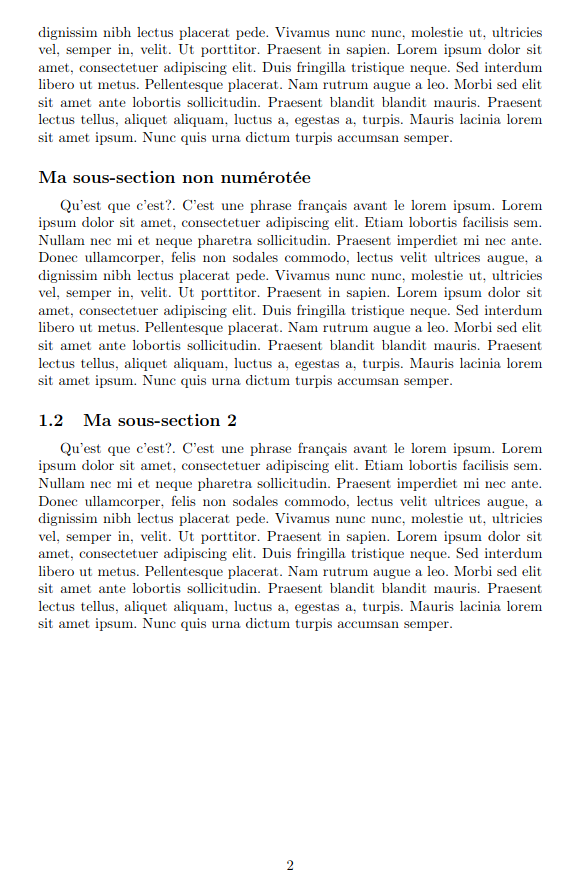
\includegraphics[scale=0.3]{ressources/testsection2}
	\end{columns}
	
\end{frame}

\begin{frame}{A vous !}
\begin{itemize}
	\item Essayez de reproduire le document ci-dessus (la forme) avec l'aide du package \texttt{blindtext}, il suffit de taper \texttt{\textbackslash blindtext} là où vous voulez écrire du texte.\\[11pt]
	\item A l'aide du package \texttt{geometry}, changez les marges de votre document en écrivant : \texttt{\textbackslash usepackage[left= , right= , top= , bottom = ]\{geometry\}}\\[11pt]
	\item Vous pouvez introduire une table des matières à tout moment en utilisant la commande \texttt{\textbackslash tableofcontents}.
\end{itemize}
\end{frame}
\section{Mise en forme}
\begin{frame}{Modifier le texte}
\begin{columns}[c]
	
	\begin{column}{0.5\textwidth}	
	\texttt{\textbackslash textbf\{gras\}}\\[11pt]
	\texttt{\textbackslash textit\{italique\}}\\[11pt]
	\texttt{\textbackslash texttt\{script\}}\\[11pt]
	\texttt{\textbackslash underline\{souligne\}}\\[11pt]
	\texttt{\textbackslash emph\{emphase\}}\\[11pt]
	\texttt{\textbackslash fbox\{encadre\}}
	\end{column}

	\begin{column}{0.5\textwidth}
	\textbf{gras}\\[11pt]
	\textit{italique}\\[11pt]
	\texttt{script}\\[11pt]
	\underline{souligne}\\[11pt]
	\emph{emphase}\\[11pt]
	\fbox{encadre}
	\end{column}
\end{columns}

\end{frame}
\begin{frame}{Faire des listes}
\begin{columns}
	\begin{column}{0.5\textwidth}
		\texttt{\textbackslash begin\{itemize\}}\\
		\texttt{\textbackslash item Item 1}\\
		\texttt{\textbackslash item Item 2}\\
		\texttt{\textbackslash item Item 3}\\
		\texttt{\textbackslash end\{itemize\}}\\[11pt]
		
		\texttt{\textbackslash begin\{enumerate\}}\\
		\texttt{\textbackslash item Numéro 1}\\
		\texttt{\textbackslash item Numéro 2}\\
		\texttt{\textbackslash item Numéro 3}\\
		\texttt{\textbackslash end\{enumerate\}}
	\end{column}
	\begin{column}{0.5\textwidth}
		\begin{itemize}
			\item Item 1
			\item Item 2
			\item Item 3\\[1cm]
		\end{itemize}
		
		\begin{enumerate}
			\item Numéro 1
			\item Numéro 2
			\item Numéro 3
		\end{enumerate}
	\end{column}
\end{columns}
\end{frame}
\begin{frame}{D'autres commandes}
\begin{itemize}
	\item Aligner son texte : \texttt{center,flushleft,flushright}.\\[11pt]
	\item Notes de bas de page : \texttt{\textbackslash footnote\{\}}.\\[11pt]
	\item Sauter une ligne : \texttt{\textbackslash \textbackslash, \textbackslash newline}.\\[11pt]
	\item Ne pas indenter un paragraphe : \texttt{\textbackslash noindent}, ou si vous voulez le faire pour tous : \texttt{\textbackslash setlength\{\textbackslash parindent\}\{0pt\}}, (début de document).
\end{itemize}
\end{frame}
\section{Ecrire des mathématiques}
\begin{frame}{Exemple de formule mathématique}
La fonctionnalité la plus populaire de \LaTeX \ est que vous pouvez écrire des formules mathématiques complexes sans problèmes par exemple:\\[11pt]

\begin{columns}
	\begin{column}{0.5\textwidth}
		\texttt{\textbackslash [ \textbackslash int\_0$\wedge$n f(t)dt = \textbackslash lim\_\{n \textbackslash to + \textbackslash +\textbackslash infty\} \textbackslash frac\{1\}\{n\} \textbackslash sum\_\{k=0\}$\wedge$\{n-1\}f(\textbackslash frac\{k\}\{n\})  \textbackslash]}
	\end{column}

	\begin{column}{0.5\textwidth}
		\[ \int_{0}^{1} f(t)dt = \lim_{n \to +\infty} \frac{1}{n}\sum_{k=0}^{n-1}f\bigg(\frac{k}{n}\bigg)\]
	\end{column}
\end{columns}
\end{frame}

\begin{frame}{Le mode math \textit{inline} vs. \textit{display}}
Deux façons d'écrire des mathématiques :\\[11pt]
\begin{itemize}
	\item Le mode \textit{inline} : \texttt{\textbackslash ( \textbackslash)} ou \texttt{\$ \$}\\[11pt].
	\item Le mode \textit{display} : \texttt{\textbackslash [ \textbackslash]} (ou \texttt{\$\$  \$\$} mais à éviter).
	\begin{columns}
		\begin{column}{0.4\textwidth}
			\[ \int_{0}^{1} f(t)dt = \lim_{n \to +\infty} \frac{1}{n}\sum_{k=0}^{n-1}f\bigg(\frac{k}{n}\bigg)\]
		\end{column}
	\hspace{1cm}
		\begin{column}{0.6\textwidth}
			\( \int_{0}^{1} f(t)dt = \lim_{n \to +\infty} \frac{1}{n}\sum_{k=0}^{n-1}f(\frac{k}{n}) \)
		\end{column}
	\end{columns}
\end{itemize}
\end{frame}
\begin{frame}{Des paquets utiles}
En préambule, importer les paquets \texttt{amsmath} et \texttt{mathtools}
\end{frame}
\begin{frame}[fragile]{Les commandes mathématiques}
\begin{columns}
	\begin{column}{0.5\textwidth}
		\verb|\frac{num}{den}|\\[11pt]
		\verb|base^{exposant}|\\[11pt]
		\verb|base_{indice}|\\[11pt]
		\verb|\sum_{bas}^{haut} expression|\\[11pt]
		\verb|\int_{min}^{max}|\\[11pt]
		\verb|\sqrt[n]{nombre}|\\[11pt]
		\verb|\lim_{x \to a}|
	\end{column}
\hspace{0.5cm}
	\begin{column}{0.5\textwidth}
		$\frac{num}{den}$\\[11pt]
		$base^{exposant}$\\[11pt]
		$base_{indice}$\\[11pt]
		$\sum_{bas}^{haut} expression$\\[11pt]
		$\int_{min}^{max}$\\[11pt]
		$\sqrt[n]{nombre}$\\[11pt]
		$\lim_{x \to a}$
	\end{column}
\end{columns}
\end{frame}

\begin{frame}[fragile]{Les symboles}
Les lettres grecques\\[11pt]

\begin{columns}
	\begin{column}{0.5\textwidth}
		\verb|\alpha, \beta, \gamma|\\
		\verb|\Omega, \Lambda, \Psi|
	\end{column}
	\begin{column}{0.5\textwidth}
		$\alpha \quad \beta \quad \gamma$\\
		$\Omega \quad \Lambda \quad \Psi$\\[11pt]
	\end{column}
\end{columns}
\vfill
Les glyphes mathématiques:\\[11pt]
\begin{columns}
	\begin{column}{0.5\textwidth}
		\verb|\forall \exists \in|\\
		\verb|\to \infty \partial|\\
		\verb|\mathbb{R} \mathcal{C} \mathbf{I}|
	\end{column}
	\begin{column}{0.5\textwidth}
		\begin{center}
			$\forall \quad \exists \quad \in$\\
			$\to \quad \infty \quad \partial$\\
			$\mathbb{R} \quad \mathcal{C} \quad \mathbf{I}$
		\end{center}
		
	\end{column}
\end{columns}
\end{frame}
\begin{frame}[fragile]{Faire des équations}
Avec l'environnement \texttt{equation}:\\[11pt]
\begin{columns}
	\begin{column}{0.5\textwidth}
	\verb|\begin{equation}|\\
	\verb|\cos^2(x)+\sin^2(x) = 1|\\
	\verb|\end{equation}|	
\end{column}
\begin{column}{0.5\textwidth}
\begin{equation}
\cos^2(x)+\sin^2(x) = 1
\end{equation}\end{column}
\end{columns}
Avec l'environnement \texttt{align} :\\[11pt]
\begin{columns}
	\begin{column}{0.5\textwidth}
\verb|\begin{align}|\\
\verb|f(x) & = 3x^2 + x\\|\\
\verb| & = (3x+1)x|\\
\verb|\end{align}|	

\end{column}
\begin{column}{0.5\textwidth}
\begin{align}
f(x) & = 3x^2 + x\\
& = (3x+1)x
\end{align}
\end{column}
\end{columns}
\vfill
$\rightarrow$ Vous pouvez toujours ajouter un \texttt{*} au nom de l'environnement pour enlever la numérotation.
\end{frame}
\begin{frame}{A vous !}

\end{frame}
\section{Présenter ses résultats}
\begin{frame}[fragile]{Faire des références}
	Association \texttt{\textbackslash label\{label\}} et \texttt{\textbackslash ref\{label\}}, à mettre après une section, dans une équation, image, tableau, ...\\[11pt]
	\verb|\section{Ma section}|\\
	\verb|\label{surnom}|\\[11pt]
	\verb|\section{Ma deuxième section}|\\[11pt]
	\verb|Je fais référence a la section \ref{surnom}|
	
\end{frame}
\begin{frame}[fragile]{Inclure des images}
Importer le paquet \texttt{graphicx}.\\[11pt]
\verb|\begin{figure}[h!]|\\
\verb|\label{mon_image}|\\
\verb|\centering|\\
\verb|\includegraphics[scale=x]{chemin/vers/mon/image.png}|\\
\verb|\caption{Ma légende}|\\
\verb|\end{figure}|
\end{frame}

\end{document}
